\let\negmedspace\undefined
\let\negthickspace\undefined
\documentclass[journal]{IEEEtran}
\usepackage[a5paper, margin=10mm, onecolumn]{geometry}
\usepackage{lmodern} % Ensure lmodern is loaded for pdflatex
\usepackage{tfrupee} % Include tfrupee package

\setlength{\headheight}{1cm} % Set the height of the header box
\setlength{\headsep}{0mm}     % Set the distance between the header box and the top of the text
\newcommand\hmmax{0}
\newcommand\bmmax{0}
\usepackage{gvv-book}
\usepackage{gvv}
\usepackage{cite}
\usepackage{amsmath,amssymb,amsfonts,amsthm}
\usepackage{algorithmic}
\usepackage{graphicx}
\graphicspath{{./figs/}}
\usepackage{textcomp}
\usepackage{xcolor}
\usepackage{txfonts}
\usepackage{listings}
\usepackage{enumitem}
\usepackage{mathtools}
\usepackage{gensymb}
\usepackage{comment}
\usepackage[breaklinks=true]{hyperref}
\usepackage{tkz-euclide} 
\usepackage{listings}
\usepackage{gvv}                                        
\def\inputGnumericTable{}                                 
\usepackage[latin1]{inputenc}                                
\usepackage{color}                                            
\usepackage{array}                                            
\usepackage{longtable}                                       
\usepackage{calc}                                             
\usepackage{multirow}                                         
\usepackage{hhline}                                           
\usepackage{ifthen}                                           
\usepackage{lscape}
\usepackage{circuitikz}
\tikzstyle{block} = [rectangle, draw, fill=blue!20, 
text width=4em, text centered, rounded corners, minimum height=3em]
\tikzstyle{sum} = [draw, fill=blue!10, circle, minimum size=1cm, node distance=1.5cm]
\tikzstyle{input} = [coordinate]
\tikzstyle{output} = [coordinate]


\begin{document}
	
	\bibliographystyle{IEEEtran}
	\vspace{3cm}
	
	\title{1.10.17}
	\author{EE25BTECH11054 - Soma Harsha Vardhan Reddy }
	\maketitle
	% \newpage
	% \bigskip
	{\let\newpage\relax\maketitle}
	
	\renewcommand{\thefigure}{\theenumi}
	\renewcommand{\thetable}{\theenumi}
	\setlength{\intextsep}{10pt} % Space between text and floats
	
	
	\numberwithin{equation}{enumi}
	\numberwithin{figure}{enumi}
	\renewcommand{\thetable}{\theenumi}
	
	\textbf{Question}:\\
    Find the unit vector in the direction of the sum of the vectors, 
    $\vec{a} = 2\vec{i}+2\vec{j}-5\vec{k} $ and $\vec{b} = 2\vec{i}+\vec{j}+3\vec{k} $

    \solution \\
    Given the vectors $\vec{a}  \text{ and } \vec{b}$
    \begin{align}
		\vec{a} = \begin{myvec}{2\\2\\-5} \end{myvec} , \vec{b} = \begin{myvec}{2\\1\\3} \end{myvec}
	\end{align}
    \begin{align}
	\vec{P} =	\vec{a}+\vec{b}
	\end{align}
    \begin{align}
	\vec{P} =  \begin{myvec}{4\\3\\-2} \end{myvec} 
	\end{align}
    The formula for finding unit vector along a given vector we use
    
    \begin{align}
	\vec{p} = \frac{\vec{P}}{\norm{\vec{P}}} \label{0.4}
	\end{align}
    \begin{align}
    {\norm{\vec{P}}^2} = \vec{P}^{\mathsf{T}}\vec{P}
    =\myvec{4 & 3 & -2}
    \myvec{4\\3\\-2}=29
    \end{align}
    \begin{align}
	\vec{p} = \frac{1}{\sqrt{29}}\begin{myvec}{4\\3\\-2} \end{myvec} 
	\end{align}
    
    \begin{align}
	 \vec{p} = \myvec{\frac{4}{\sqrt{29}}\\\frac{3}{\sqrt{29}}\\\frac{-2}{\sqrt{29}}}  
	\end{align}
    
\begin{figure}[H]
    \centering
    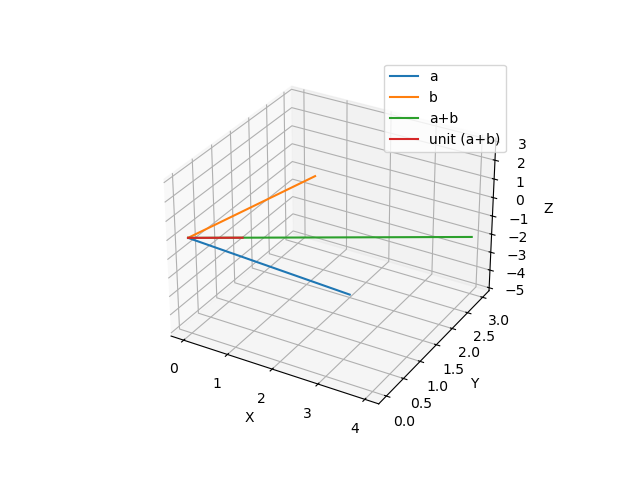
\includegraphics{figs/plot.png}
    \caption*{}
    \label{fig:plot}
\end{figure}    

\end{document}
